\documentclass{article}
    
\usepackage{Haust2017skil}

\title{Stærðfræðimynstur í tölvunarfræði \\ Skilaverkefni 3}
\author{}

\begin{document}
\maketitle

Skila skal þessu verkefni á vefnum \href{https://gradescope.com/courses/9487}{Gradescope}. Aðgangskóði fyrir námskeiðið er \textbf{9N834D}.

Gradescope tekur við .pdf skjölum. Frágangur á þeim skiptir máli. Þau skulu að vera hreinskrifuð í tölvu. Kerfi eins og \LaTeX, Google Docs og Microsoft Word geta búið til .pdf skjöl.

Samvinna á milli nemenda er eðlileg og æskileg. Hins vegar er afritun það aldrei. Miklu gagnlegra er að reyna við dæmin upp á eigin spýtur en að reyna að hala inn hærri einkunn með því að skila inn lausnum annarra.

Telji nemandi að mistök hafi verið gerð við yfirferð skal tilkynna slíkt á Gradescope.

\section{Kafli 2.4}

\question

Launþegi nokkur var ráðinn árið 2009 og fékk þá \$50,000 í árslaun. Á hverju ári hækka laun viðkomandi um \$1,000 að viðbættum 5\% af árslaunum ársins á undan.

\begin{enumerate}[a)]
    \item Setjið upp rakningarvensl sem lýsa þessum launum $n$ árum eftir 2009.
    \item Hver eru þessi laun í dag, árið 2017?
    \item Finnið formúlu á lokuðu sniði fyrir launin $n$ árum eftir 2009.
\end{enumerate}

\paragraph{Í bók} Dæmi 2.4.22 í Icelandic edition, dæmi 2.4.12 í Global edition.

\question

\textbf{(Ísl)} Finnið reglu eða formúlu til að mynda eftirfarandi runur. Notið svo regluna til að reikna út næstu þrjá liði rununnar. \textbf{(En)}  For each of these lists of integers, provide a simple formula or rule that generates the terms of an integer sequence that begins with the given list. Determine the next three terms of the sequence.


\begin{itemize}
    \item[b)] 7, 11, 15, 19, 23, 27, 31, 35, 39, 43, \ldots
    \item[d)] 1, 2, 2, 2, 3, 3, 3, 3, 3, 5, 5, 5, 5, 5, 5, 5, \ldots
    \item[e)] 0, 2, 8, 26, 80, 242, 728, 2186, 6560, 19682, \ldots
    \item[h)] 2, 4, 16, 256, 65536, 4294967296 \ldots
\end{itemize}

\paragraph{Í bók} Dæmi 2.4.26 í Icelandic edition.

\section{Kafli 2.5}

\question

Dæmi af miðmisserisprófi 2016.

\textbf{(Ísl)} Sýnið að hlutmengi teljanlegs mengis sé teljanlegt mengi.

\textbf{(En)} Show that the subset of a countable set is a countable set.

\section{Kafli 2.6}

\question Séu $A$ og $B$ $n \times n$ fylki þar sem $AB = BA = I_n$ er $B$ kölluð andhverfa (e. \emph{inverse}) $A$.

Sýnið að 
\[
    \begin{bmatrix}
        \phantom{-}2&\phantom{-}3&-1\\
        \phantom{-}1&\phantom{-}2&\phantom{-}1\\
        -1&-1&\phantom{-}3\\
    \end{bmatrix}
\]
sé andhverfa fylkisins
\[
    \begin{bmatrix}
        \phantom{-}7&-8&\phantom{-}5\\
        -4&\phantom{-}5&-3\\
        \phantom{-}1&-1&\phantom{-}1\\        
    \end{bmatrix}
\]

\paragraph{Í bók:} Dæmi 2.6.18 í báðum útgáfum.

\section{Kafli 3.1}

\question

Eftirfarandi reiknirit vantar nauðsynlega eiginleika (sjá upptalningu eftir Algorithm 1 í kennslubók, og glæru í fyrirlestri). Hvaða eiginleikar eru það, í hverju tilviki um sig?

\begin{center}
    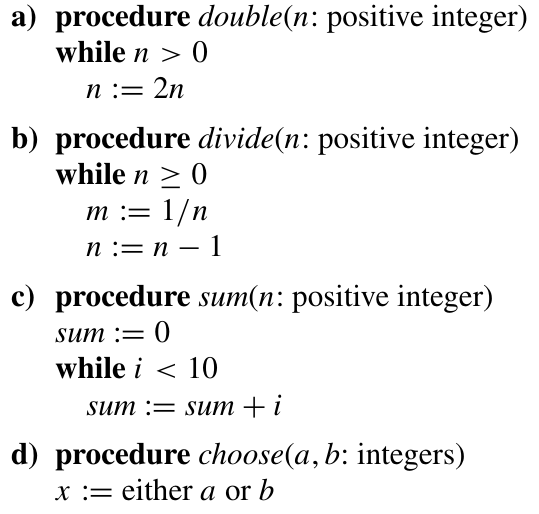
\includegraphics[width=0.4\textwidth]{badalgos}
\end{center}

\paragraph{Í bók:} 3.1.2 í báðum útgáfum.

\question

Sýnið að gráðuga myntskiptireikniritið virkar ekki þegar myntgildin eru 1, 5, 10, 12 og 25.

\paragraph{Í bók:} 3.1.56 í Icelandic edition, 3.1.46 í Global edition

\end{document}
